%%%%%%%%%%%%%%%%%%%%%%%%%%%%%% -*- Mode: Latex -*- %%%%%%%%%%%%%%%%%%%%%%%%%%%%
%% kdeTools.tex ---
%% Author          : Per Andreas Brodtkorb
%% Created On      : Sun Jul 04 13:55:59 2004
%% Last Modified By: Per Andreas Brodtkorb
%% Last Modified On: Tue May 06 16:49:07 2008
%% Last Modified By: Georg Lindgren
%% Last Modified On: April 10, 2009
%% Update Count    : 33
%% Status          : Unknown, Use with caution!
%%%%%%%%%%%%%%%%%%%%%%%%%%%%%%%%%%%%%%%%%%%%%%%%%%%%%%%%%%%%%%%%%%%%%%%%%%%%%%%
%\svnInfo $Id: kdeTools.tex 66 2017-09-05 07:01:50Z Georg Lindgren $ 
%$
%
\chapter{Kernel density estimation}
\label{cha:KDE}

Histograms are among the most popular ways to visually present data.
They are particular examples of density estimates and their appearance
depends on both the choice of origin and the width of the intervals
(bins) used. In order for the histogram to give useful information
about the true underlying distribution, a sufficient amount of data is
needed.  This is even more important for histograms in two dimensions or
higher. Also the discontinuity of the histograms may cause problems,
 \eg{,} if derivatives of the estimate are required.

An effective alternative to the histogram is the kernel density estimate (KDE),
which may be considered as a ``smoothed histogram'', only depending on
the bin-width and not depending on the origin, see
\cite{Silverman1986Density}.

\section{The univariate kernel density estimator}
The univariate KDE is defined by
\begin{equation}
  \label{eq:kdeformula}
  \hat{f}_{X}(x;h_{s}) = \frac{1}{n\,h_{s}}
                         \sum_{j=1}^{n} K_{d}\left( \frac{x-X_{j}}{h_{s}}\right),
\end{equation}
where $n$ is the number of datapoints, $X_{1},X_{2},\ldots,X_{n}$, is the
 data set, and $h_{s}$ is the smoothing parameter or window width. The
 kernel function $K_{d}$ is usually a unimodal, symmetric probability
 density function. This ensures that the KDE itself is also a density.
However, kernels that are not densities are also sometimes used
 \citep[see][]{WandAndJones1995Kernel}, but these are
not implemented in the \progname{} toolbox. \index[xentr]{window!width}
\index[xentr]{smoothing parameter}

To illustrate the method, consider the kernel estimator as a sum of
``bumps'' placed at the observations. The shape of the bumps are given
by the kernel function while the width is given by the smoothing
parameter, $h_{s}$. Fig.~\ref{fig:kdedemo1} shows a KDE constructed
 using 7 observations from a standard Gaussian distribution with a
 Gaussian kernel function. One should note that the 7 points used
 here, is purely for clarity in
 illustrating how the kernel method works. Practical density
 estimation usually involves much higher number of observations.

 Fig.~\ref{fig:kdedemo1} also demonstrates the effect of varying
 the smoothing parameter, $h_{s}$. A too small value for $h_{s}$ may introduce
 spurious bumps in the resulting KDE (top), while a too large value
 may obscure the details of the underlying distribution (bottom).
 Thus the choice of value for the smoothing parameter,
 $h_{s}$, is very important. How to select one will be elaborated
 further in the next section.

\begin{figure}[!p]
  \begin{minipage}[b]{\linewidth}%
%    \psfrag{Density}[B][t]{Density}
    \centering 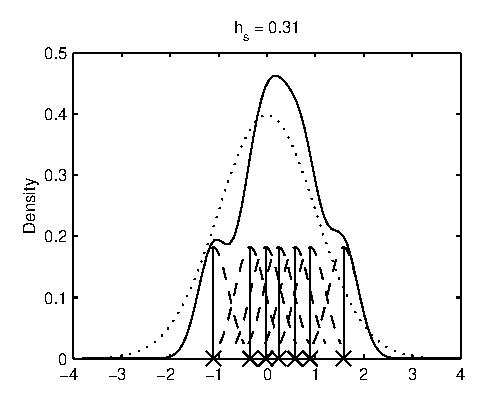
\includegraphics[height=2.5in,angle=0]{kdedemo1f1}
  \end{minipage} %%\hspace{1cm}
\vfill
  \begin{minipage}[b]{\linewidth}%
%    \psfrag{Density}[B][t]{Density}
    \centering 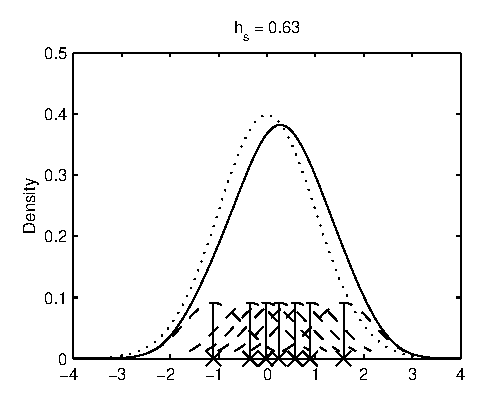
\includegraphics[height=2.5in,angle=0]{kdedemo1f2}
  \end{minipage} %%\hspace{1cm}
\vfill
  \begin{minipage}[b]{\linewidth}%
%    \psfrag{Density}[B][t]{Density}
    \centering  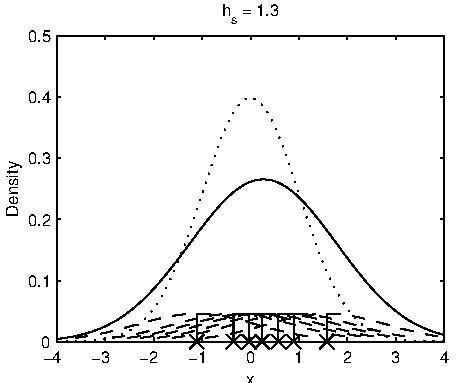
\includegraphics[height=2.5in,angle=0]{kdedemo1f3}
  \end{minipage} %%\hspace{1cm}
  \caption[Smoothing parameter, $h_{s}$, impact on KDE]{Smoothing
    parameter, $h_{s}$, impact on KDE:
    True density (dotted) compared to KDE based on 7 observations
    (solid) and their individual kernels (dashed). }  \label{fig:kdedemo1}
\end{figure}


The particular choice of kernel function, on the other hand, is
not very important since suboptimal kernels are not suboptimal by
very much, \citep[see][pp.\ 31]{WandAndJones1995Kernel}.
However, the kernel that minimizes the
mean integrated square error is the Epanechnikov kernel, and
is thus chosen as the default kernel in the software, see
Eq.~(\ref{eq:multivariateEpan}).
For a discussion of other kernel functions and their properties,
see \cite{WandAndJones1995Kernel}. \index[xentr]{Epanechnikov kernel}


\subsection{Smoothing parameter selection}
The choice of smoothing parameter,
$h_{s}$, is very important, as exemplified in Fig.\ref{fig:kdedemo1}.
In many situations it is satisfactory to select the smoothing
parameter subjectively by eye, \ie{} look at several density
estimates over a range of bandwidths and selecting the density that is
the most ``pleasing'' in some sense.
However, there are also many  circumstances where it is beneficial to
use an automatic bandwidth selection from the data. One reason is that
it is very time consuming to select the bandwidth by eye.
Another reason, is that,
in many cases, the user has no prior knowledge of the
structure of the data, and does not have any feeling for which
bandwidth gives a good estimate. One simple, quick and commonly used
automatic bandwidth selector, is the bandwidth that minimizes the mean
integrated square error (MISE) asymptotically. As shown in
\cite[Section 2.5 and 3.2.1]{WandAndJones1995Kernel}, the one dimensional
AMISE\footnote{AMISE = asymptotic mean integrated square error}-optimal normal
scale rule assuming that the underlying density is Gaussian, is given by

\begin{equation}
  \label{eq:Hamise}
  h_{AMISE} =
  %  \left[\frac{8\,\sqrt{\pi}\,R(K_{d})}{3\,\mu_{2}^{2}(K_{d})
  %\,n}\right]^{1/5}\,\widehat{\sigma} =
\left[\frac{4}{3\,n}\right]^{1/5}\,\widehat{\sigma} ,
\end{equation}
where $\widehat{\sigma}$ is some estimate of the standard deviation of the
underlying distribution. Common choices of $\widehat{\sigma}$ are the
sample standard deviation, $\widehat{\sigma}_{s}$, and the standardized
interquartile range (denoted IQR):
\begin{equation}
  \label{eq:Oiqr}
  \widehat{\sigma}_{IQR} = (\text{sample IQR})/
  (\Phi^{-1}(3/4)-\Phi^{-1}(1/4)) \approx  (\text{sample IQR})/1.349 ,
\end{equation}
where $\Phi^{-1}$ is the standard normal quantile function. The use of
$\widehat{\sigma}_{IQR}$ guards against outliers if the distribution has
heavy tails.
A reasonable approach is to use the smaller of $\widehat{\sigma}_{s}$ and
$\widehat{\sigma}_{IQR}$ in order to lessen the chance of oversmoothing,
\cite[see][pp.\ 47]{Silverman1986Density}.

Various other automatic methods for selecting $h_{s}$ are available and are
discussed in \cite{Silverman1986Density} and in more detail in
\cite{WandAndJones1995Kernel}.

\subsection{Transformation kernel denstity estimator}
%The Gaussian distribution is one of the easiest distributions to
%obtain a good KDE from \citep[][Chap. 2.9]{WandAndJones1995Kernel}.
Densities close to normality appear to be the easiest for
the kernel estimator to estimate. The estimation
difficulty increases with skewness, kurtosis and multimodality
\citep[][Chap. 2.9]{WandAndJones1995Kernel}.

Thus, in the cases where the random sample $X_{1},X_{2},\ldots,X_{n}$,
has a density, $f$, which is difficult to estimate, a transformation, $t$,
might give a good KDE, \ie{} applying a transformation to the data to obtain
a new sample $Y_{1},Y_{2},\ldots,Y_{n}$, with a density $g$ that
more easily can be estimated using the basic KDE. One would then
backtransform the estimate of $g$ to obtain the estimate for $f$.

Suppose that $Y_{i} = t(X_{i})$, where $t$ is an increasing
differentiable function defined on the support of $f$. Then a standard
result from statistical distribution theory is that
\begin{equation}
  \label{eq:transform}
  f(x) = g(t(x))\,t'(x),
\end{equation}
where $t'(x)$ is the derivative.
Backtransformation of the KDE of $g$ based on
$Y_{1},Y_{2},\ldots,Y_{n}$, leads to the explicit formula
\begin{equation}
  \label{eq:transformkdeformula}
  \hat{f}_{X}(x;h_{s},t) = \frac{1}{n\,h_{s}} \sum_{j=1}^{n}
K_{d}\left( \frac{t(x)-t(X_{j})}{h_{s}}\right)\,t'(x)
\end{equation}

A simple illustrative example comes from the problem of
estimating the Rayleigh density. This density is very difficult to
estimate by direct kernel methods. However, if we apply the
transformation $Y_{i} = \sqrt{X_{i}}$ to the data, then the normal plot
of the transformed data, $Y_{i}$, becomes approximately linear.
Fig.~\ref{fig:transformkde} shows that the transformation KDE is a
better estimate around 0 than the ordinary KDE.
\begin{figure}[htb]
  \begin{minipage}[b]{0.5\linewidth}%
%    \psfrag{Density}[B][t]{Density}
    \centering  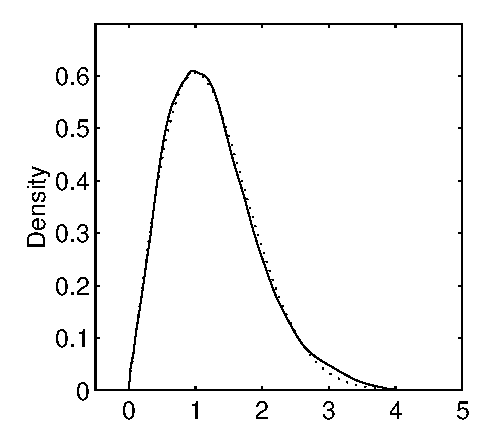
\includegraphics[width=2.5in]{rayleightransformedkde}
  \end{minipage} \hfill %%\hspace{1cm}
  \begin{minipage}[b]{0.5\linewidth}%
%    \psfrag{Density}[B][t]{Density}
    \centering 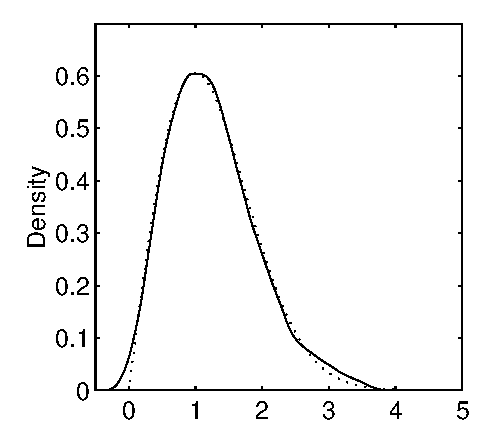
\includegraphics[width=2.5in]{rayleighkde}
  \end{minipage} %%\hspace{1cm}
  \caption[Transformation KDE compared to ordinary KDE]
        {True Rayleigh density (dotted) compared to transformation
        KDE (solid,left) and ordinary KDE (solid, right) based on 1000 observations.}
\label{fig:transformkde}
\end{figure}

\section{The multivariate kernel density estimator}
\label{sec:multivariateKDE}
The multivariate kernel density estimator is defined in its most
general form by
\begin{equation}
  \label{eq:multivariateKDE}
  \widehat{f}_{\mbf{X}}(\mbf{x};\mbf{H}) = \frac{|\mbf{H}|^{-1/2}}{n}
 \sum_{j=1}^{n} K_{d}\left(\mbf{H}^{-1/2}(\mbf{x}-\mbf{X}_{j})\right),
\end{equation}
where $\mbf{H}$ is a symmetric positive definite $d \times d$ matrix
called the \textit{bandwidth matrix}. \index[xentr]{bandwidth matrix}
A simplification of
Eq.~(\ref{eq:multivariateKDE}) can be obtained by imposing the
restriction $\mbf{H} = \text{diag}(h_{1}^{2}, h_{2}^{2}, \ldots ,
h_{d}^{2})$. Then Eq.~(\ref{eq:multivariateKDE}) reduces to
\begin{equation}
  \label{eq:multivariateKDE2}
  \widehat{f}_{\mbf{X}}(\mbf{x};\mbf{h}) =
  \frac{1}{n\,\prod_{i=1}^{n}\,h_{i}}
  \sum_{j=1}^{n} K_{d}\left(\frac{x-X_{j\,1}}{h_{1}},
    \frac{x-X_{j\,2}}{h_{2}},\ldots,
    \frac{x-X_{j\,d}}{h_{d}} \right),
\end{equation}
and is, in combination with a transformation, a reasonable solution
to visualize multivariate densities.

The multivariate Epanechnikov kernel also forms the basis for the
optimal spherically symmetric multivariate kernel
and is given by \index[xentr]{Epanechnikov kernel!multivariate}
\begin{equation}
  \label{eq:multivariateEpan}
  K_{d}(\mbf{x}) = \frac{d+2}{2\,v_{d}}
  \left(1-\mbf{x}^{T}\mbf{x} \right)\mbf{1}_{\mbf{x}^{T}\mbf{x}\le 1},
\end{equation}
where $v_{d}=2\,\pi^{d/2}/( \Gamma(d/2) \, d )$ is the volume of the unit
$d$-dimensional sphere.

In this tutorial we use the KDE to find a good estimator of the
central part of
the joint densities of wave parameters extracted from time series.
Clearly, such data are dependent,
so it is assumed that the time series
are ergodic and short range dependent to justify the use of
KDE:s, \citep[see][Chap. 6]{WandAndJones1995Kernel}.
Usually, KDE gives poor estimates of the tail of
the distribution, unless large amounts of data is available. However,
a KDE gives qualitatively good estimates in the regions of sufficient
data, \ie{} in the main parts of the distribution. This is good for
visualization, \eg{} detecting modes, symmetries of distributions.

%http://science.ntu.ac.uk/maths.html
The kernel density estimation software is 
based on  {\tt KDETOOL}, which is a \ML{} toolbox produced by
Christian Beardah, \cite{BeardahBaxter1996},
%\footnote{See \href{http://science.ntu.ac.uk/msor/ccb/densest.html}{http://science.ntu.ac.uk/msor/ccb/densest.html}} 
which has been 
%However, over the past 10 years the toolbox is
 totally rewritten and extended
to include the transformation kernel estimator and generalized to cover
any dimension for the data. The computational speed has also been improved.



%%% Local Variables:
%%% mode: latex
%%% TeX-master: "wafomanual"
%%% End:
